% ---------------------------------------------------------------------------
% diagrams.tex — diagram slides and their layout helpers
%
% Kept apart from content.tex because the diagrams are drawn separately: each
% macro here can be replaced on its own, or a frame in content.tex can be
% swapped for a plain placeholder, without touching the surrounding slides.
%
%   \systemOverviewSlide   block diagram
%   \clientFlowchartSlide  client flowchart
%   \serverFlowchartSlide  server flowchart
%   \dataFlowSlide         data flow diagram
%   \columnsimage{...}     a console screenshot with its caption
% ---------------------------------------------------------------------------

% --- a screenshot with its caption, side by side ---------------------------

% #1 asset name (in assets/), #2 image width, #3 caption text
%
% Both dimensions are capped. The screenshots are all 960x570, so a width that
% fills the column would stand taller than the frame once the caption is
% beside it; the caption is set small for the same reason.
\newcommand{\columnsimage}[3]{%
  \begin{columns}[c, onlytextwidth]
    \begin{column}{0.62\textwidth}
      \includegraphics[width=\linewidth, height=0.50\textheight,
                       keepaspectratio]{assets/#1}
    \end{column}
    \begin{column}{0.36\textwidth}
      {\scriptsize #3}
    \end{column}
  \end{columns}%
}

% --- 1. System overview: block diagram -------------------------------------


% ===========================================================================
% The four architecture diagrams
%
% These are the real ones, supplied as standalone TikZ documents at the top of
% this folder (project BD.tex, client2.tex, server.tex, dataflow.tex). Each is
% built to a one-page PDF in diagrams/ and included here whole, rather than
% redrawn inline -- the originals stay the single source and can be edited and
% recompiled without touching the deck.
%
% They are wide (25-31 cm at natural size), so each is fitted to the slide:
% full text width where that also clears the height, otherwise capped by
% height and centred. Both bounds are given to \includegraphics so the smaller
% of the two wins and the aspect ratio is never distorted.
% ===========================================================================

% --- block diagram: client, server, worker pool, shared region --------------

\newcommand{\systemOverviewSlide}{%
\begin{frame}{System Architecture}
  \begin{center}
    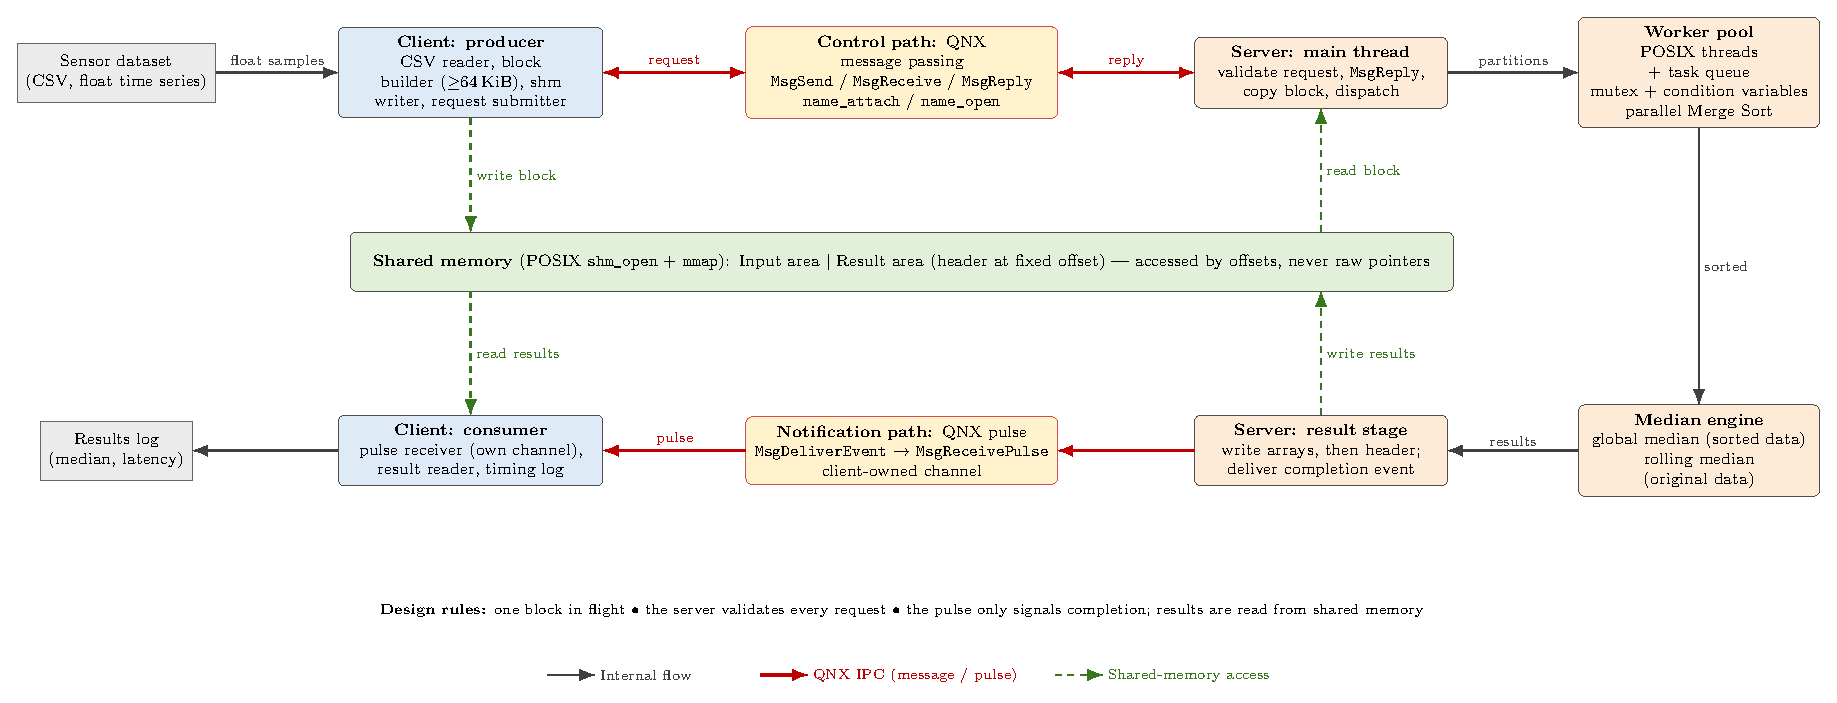
\includegraphics[width=\textwidth, height=0.78\textheight,
                     keepaspectratio]{diagrams/project BD.pdf}
  \end{center}
\end{frame}%
}

% --- client side -----------------------------------------------------------

\newcommand{\clientFlowchartSlide}{%
\begin{frame}{Client: Connect, Offload, Collect}
  \begin{center}
    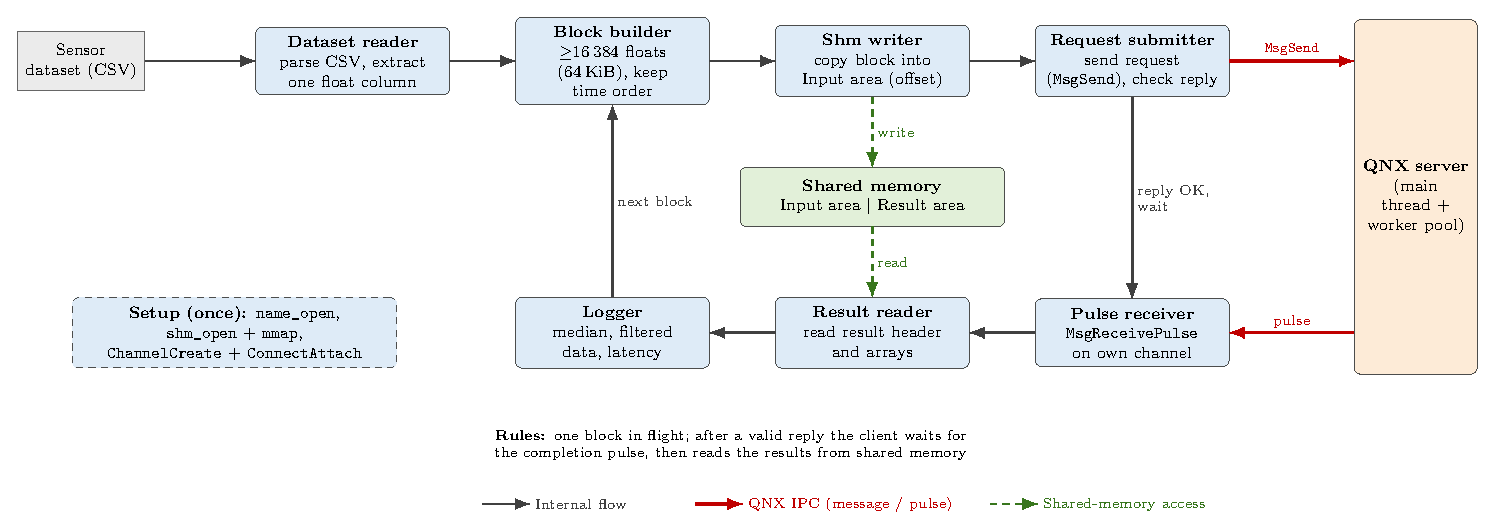
\includegraphics[width=\textwidth, height=0.78\textheight,
                     keepaspectratio]{diagrams/client2.pdf}
  \end{center}
\end{frame}%
}

% --- server side -----------------------------------------------------------

\newcommand{\serverFlowchartSlide}{%
\begin{frame}{Server: Accept, Validate, Answer}
  \begin{center}
    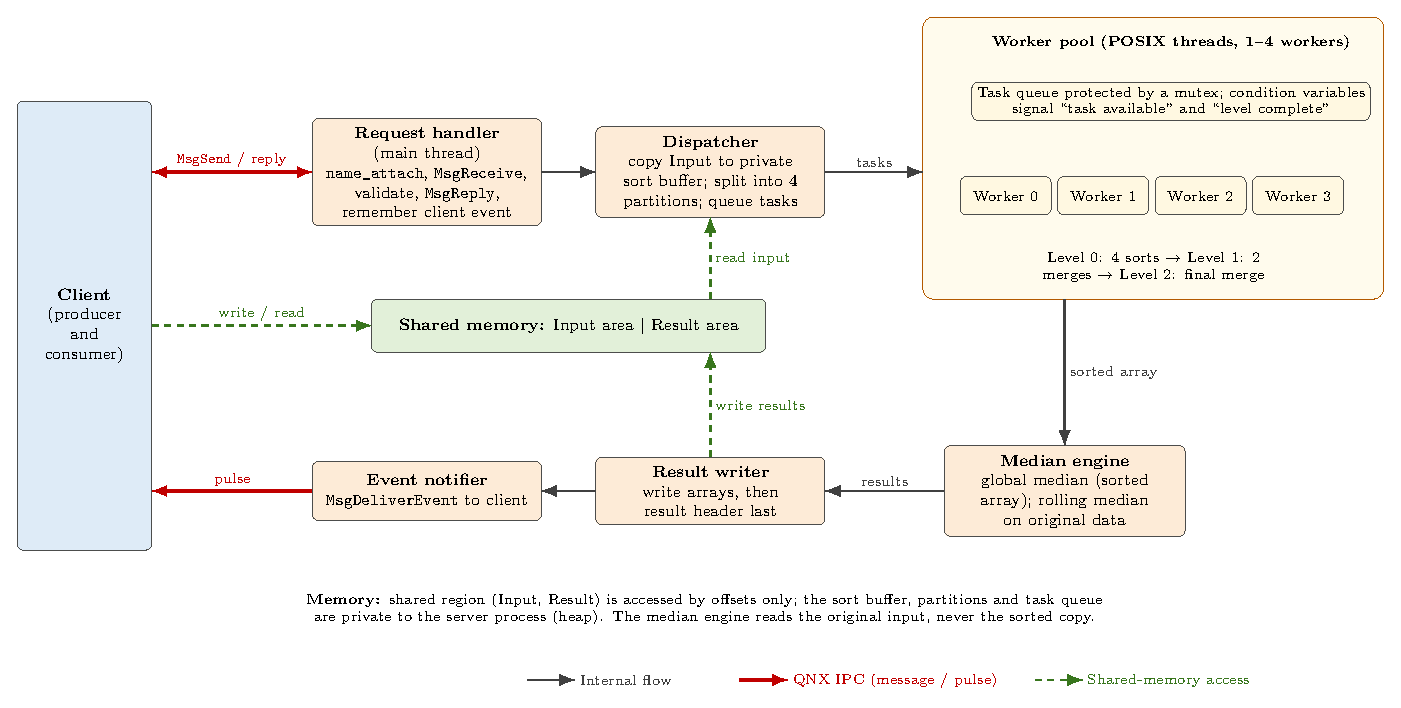
\includegraphics[width=\textwidth, height=0.78\textheight,
                     keepaspectratio]{diagrams/server.pdf}
  \end{center}
\end{frame}%
}

% --- data flow -------------------------------------------------------------

\newcommand{\dataFlowSlide}{%
\begin{frame}{Data Flow}
  \begin{center}
    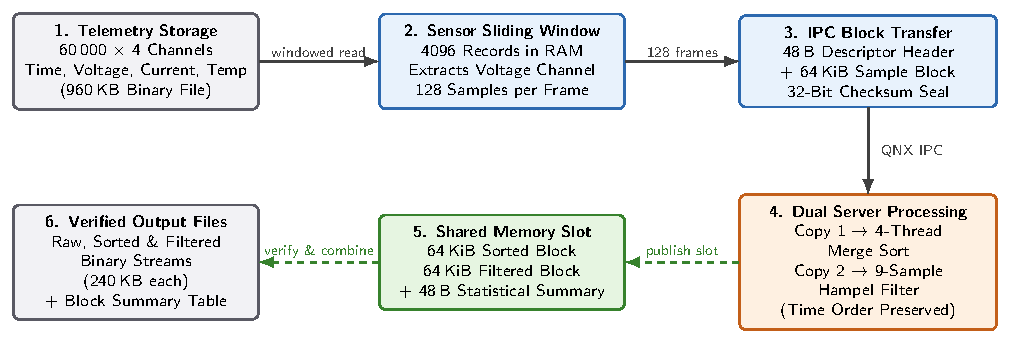
\includegraphics[width=\textwidth, height=0.78\textheight,
                     keepaspectratio]{diagrams/dataflow.pdf}
  \end{center}
\end{frame}%
}
